\chapter{The Distance Formula using pythagoras}
\noindent
% --- EDITOR VISIBILITY CHECK ---
% If you can read this, the mobile editor is working.
\colorbox{practicegreen}{\parbox{\dimexpr\linewidth-2\fboxsep}{\centering\small\bfseries\color{white} EXPERIMENTAL LAB: FIELD APPLICATIONS}}
\vspace{15pt}

\begin{enumerate} 
    \item \textbf{LaserRangefinderCalibration:} A surveyor places a laser at origin $(0,0)$ and a reflector at $(15, 20)$. The laser reads $24.8$ units. Calculate the theoretical distance and find the percentage error.
    
    \begin{center}
    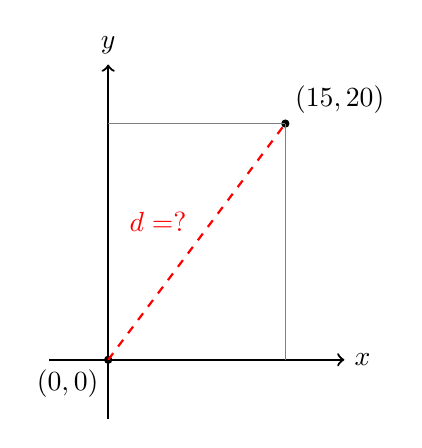
\begin{tikzpicture}[scale=0.15]
        \draw[->,thick] (-5,0) -- (20,0) node[right] {$x$};
        \draw[->,thick] (0,-5) -- (0,25) node[above] {$y$};
        \draw[fill=black] (0,0) circle (0.3) node[below left] {$(0,0)$};
        \draw[fill=black] (15,20) circle (0.3) node[above right] {$(15,20)$};
        \draw[red, thick, dashed] (0,0) -- (15,20) node[midway, above left] {$d = ?$};
        \draw[gray, thin] (15,0) -- (15,20);
        \draw[gray, thin] (0,20) -- (15,20);
    \end{tikzpicture}
    \end{center}

    \item \textbf{The Acoustic Localization:} Two microphones at $M_1(-5, 0)$ and $M_2(5, 0)$ detect sound. A third at $M_3(0, 12)$ detects it later. Find the source $S(0, y)$.
    
    \begin{center}
    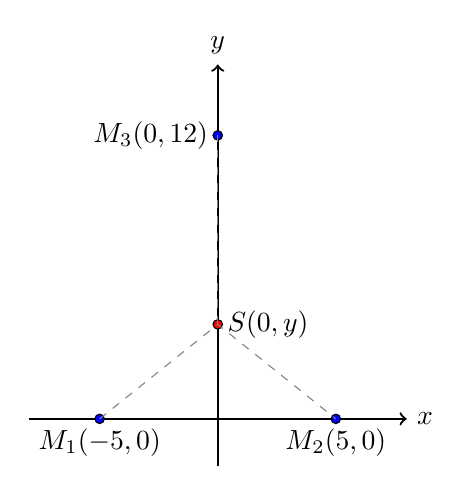
\begin{tikzpicture}[scale=0.3]
        \draw[->,thick] (-8,0) -- (8,0) node[right] {$x$};
        \draw[->,thick] (0,-2) -- (0,15) node[above] {$y$};
        \draw[fill=blue] (-5,0) circle (0.2) node[below] {$M_1(-5,0)$};
        \draw[fill=blue] (5,0) circle (0.2) node[below] {$M_2(5,0)$};
        \draw[fill=blue] (0,12) circle (0.2) node[left] {$M_3(0,12)$};
        \draw[fill=red] (0,4) circle (0.2) node[right] {$S(0,y)$};
        \draw[dashed, gray] (-5,0) -- (0,4) -- (5,0);
        \draw[dashed, gray] (0,4) -- (0,12);
    \end{tikzpicture}
    \end{center}

    \item \textbf{Shadow Tracking:} A pole's top is at $(0, 5)$ and its shadow is at $(3, 0)$. When the sun moves, the shadow moves to $(0, 0)$. Calculate the total distance the shadow tip traveled.
    
    \begin{center}
    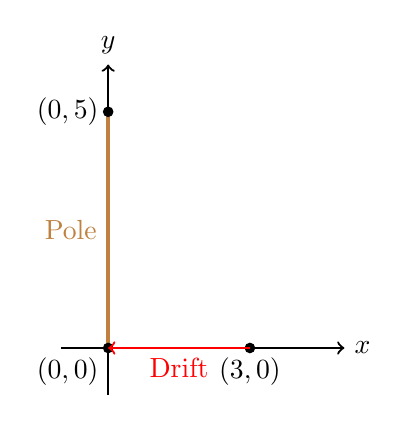
\begin{tikzpicture}[scale=0.6]
        \draw[->,thick] (-1,0) -- (5,0) node[right] {$x$};
        \draw[->,thick] (0,-1) -- (0,6) node[above] {$y$};
        \draw[ultra thick, brown] (0,0) -- (0,5) node[midway, left] {Pole};
        \draw[fill=black] (0,5) circle (0.1) node[left] {$(0,5)$};
        \draw[fill=black] (3,0) circle (0.1) node[below] {$(3,0)$};
        \draw[fill=black] (0,0) circle (0.1) node[below left] {$(0,0)$};
        \draw[red, ->, thick] (3,0) -- (0,0) node[midway, below] {Drift};
    \end{tikzpicture}
    \end{center}

    \item \textbf{Tension Wire Stability:} A tower at $(0, 12)$ is secured by wires anchored at $(x, 0)$ and $(-x, 0)$. If the total length of both wires is 26, find $x$.
    
    \begin{center}
    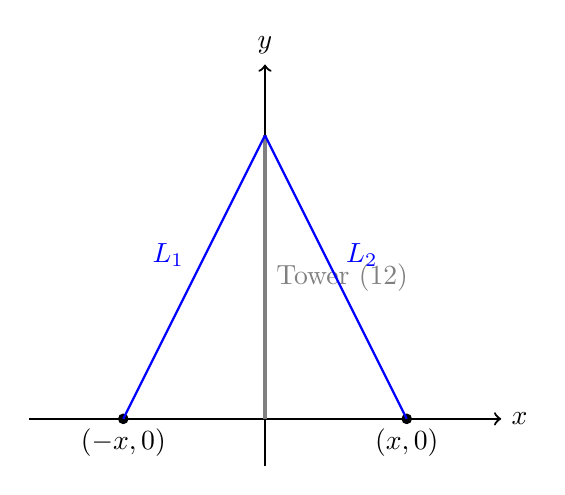
\begin{tikzpicture}[scale=0.3]
        \draw[->,thick] (-10,0) -- (10,0) node[right] {$x$};
        \draw[->,thick] (0,-2) -- (0,15) node[above] {$y$};
        \draw[ultra thick, gray] (0,0) -- (0,12) node[midway, right] {Tower (12)};
        \draw[fill=black] (6,0) circle (0.2) node[below] {$(x,0)$};
        \draw[fill=black] (-6,0) circle (0.2) node[below] {$(-x,0)$};
        \draw[thick, blue] (-6,0) -- (0,12) node[midway, above left] {$L_1$};
        \draw[thick, blue] (6,0) -- (0,12) node[midway, above right] {$L_2$};
    \end{tikzpicture}
    \end{center}

    \item \textbf{GPS Drift Analysis:} Readings at $(10, 10)$ drift to $(10.1, 9.9)$ and $(9.8, 10.2)$. Find the average distance of these drift points from the center.
    
    \begin{center}
    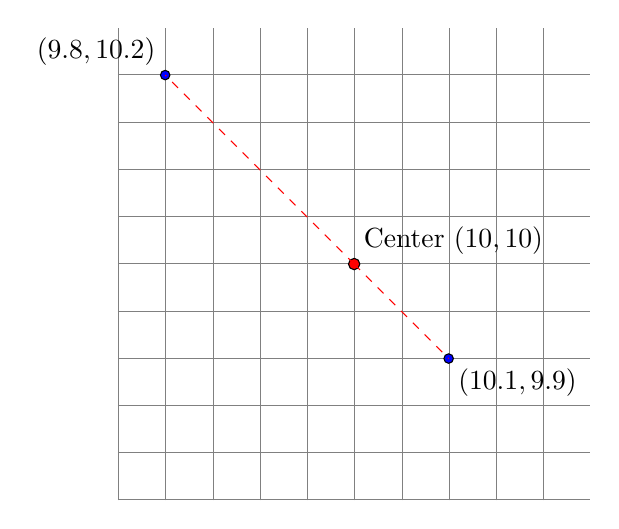
\begin{tikzpicture}[scale=12]
        \draw[step=0.05, gray, very thin] (9.75, 9.75) grid (10.25, 10.25);
        \draw[fill=red] (10,10) circle (0.006) node[above right] {Center $(10,10)$};
        \draw[fill=blue] (10.1,9.9) circle (0.005) node[below right] {$(10.1, 9.9)$};
        \draw[fill=blue] (9.8,10.2) circle (0.005) node[above left] {$(9.8, 10.2)$};
        \draw[dashed, red] (10,10) -- (10.1,9.9);
        \draw[dashed, red] (10,10) -- (9.8,10.2);
    \end{tikzpicture}
    \end{center}
\end{enumerate}

\chapter{Coordinate Geometry}
\section{Introduction}
Coordinate geometry, also known as analytic geometry, is the study of geometry using a coordinate system. This contrasts with synthetic geometry.

\section{The Cartesian Plane}
The Cartesian plane is defined by two perpendicular number lines: the x-axis, which is horizontal, and the y-axis, which is vertical.

\chapter{physics}
\noindent
% --- MODULE HEADER ---
\definecolor{labblue}{HTML}{0056B3} % Defined inline to prevent compilation errors
\colorbox{labblue}{\parbox{\dimexpr\linewidth-2\fboxsep}{\centering\small\bfseries\color{white} EXPERIMENTAL LAB: VECTOR KINEMATICS \& DYNAMICS}}
\vspace{15pt}

\begin{enumerate}
    \item \textbf{Drone Navigation Vectors:} A quadcopter flies from a launch pad with a velocity vector $\vec{v} = 8\hat{i} + 6\hat{j}$ meters per second. Calculate its total ground speed $|\vec{v}|$ and the heading angle $\theta$ relative to the positive $x$-axis.
    
    \begin{center}
    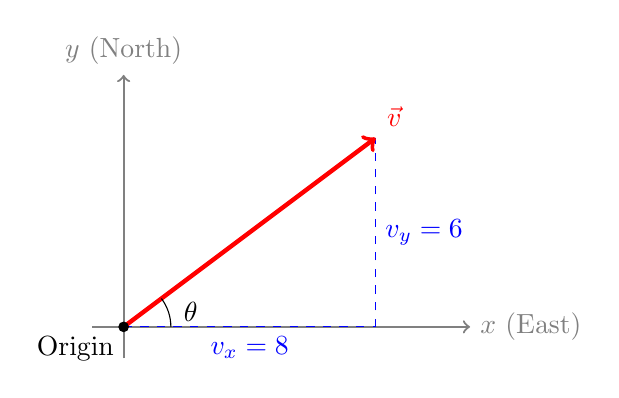
\begin{tikzpicture}[scale=0.4]
        % Axes
        \draw[->,thick,gray] (-1,0) -- (11,0) node[right] {$x$ (East)};
        \draw[->,thick,gray] (0,-1) -- (0,8) node[above] {$y$ (North)};
        % Vector components
        \draw[dashed, blue] (0,0) -- (8,0) node[midway, below] {$v_x = 8$};
        \draw[dashed, blue] (8,0) -- (8,6) node[midway, right] {$v_y = 6$};
        % Resultant Vector
        \draw[->, ultra thick, red] (0,0) -- (8,6) node[above right] {$\vec{v}$};
        % Angle arc
        \draw (1.5,0) arc (0:36.87:1.5) node[midway, right, xshift=2pt] {$\theta$};
        \draw[fill=black] (0,0) circle (0.15) node[below left] {Origin};
    \end{tikzpicture}
    \end{center}
    \vspace{10pt}

    \item \textbf{Projectile Trajectory Analysis:} A ball launcher fires a projectile from ground level at an angle of $45^\circ$ with an initial speed of $14\text{ m/s}$. Sketch the parabolic path and compute the peak vertex $(h, k)$ where vertical velocity $v_y = 0$.
    
    \begin{center}
    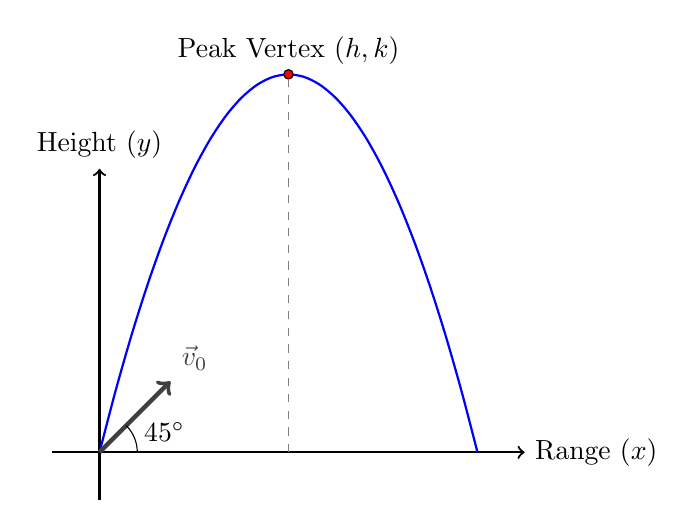
\begin{tikzpicture}[scale=0.6]
        % Axes
        \draw[->,thick] (-1,0) -- (9,0) node[right] {Range ($x$)};
        \draw[->,thick] (0,-1) -- (0,6) node[above] {Height ($y$)};
        % Parabolic path
        \draw[domain=0:8, smooth, variable=\x, thick, blue] plot ({\x}, {4*\x - 0.5*\x*\x});
        % Vertex point
        \draw[fill=red] (4,8) circle (0.1) node[above] {Peak Vertex $(h,k)$};
        \draw[dashed, gray] (4,0) -- (4,8);
        % Initial Vector arrow
        \draw[->, ultra thick, darkgray] (0,0) -- (1.5,1.5) node[above right] {$\vec{v}_0$};
        \draw (0.8,0) arc (0:45:0.8) node[midway, right, yshift=2pt] {$45^\circ$};
    \end{tikzpicture}
    \end{center}
    \vspace{10pt}

    \item \textbf{Centripetal Force Boundaries:} A tethered test vehicle undergoes uniform circular motion around a central pillar at $(0,0)$ with a fixed radius of $5\text{ meters}$. Show the direction of the centripetal acceleration vector $\vec{a}_c$ relative to the position vector $\vec{r}$.
    
    \begin{center}
    \begin{tikzpicture}[scale=0.5]
        % Coordinates and circle
        \draw[gray, dashed] (0,0) circle (5);
        \draw[->,thick] (-6,0) -- (6,0) node[right] {$x$};
        \draw[->,thick] (0,-6) -- (0,6) node[above] {$y$};
        % Object position at 30 degrees (R=5 -> x=4.33, y=2.5)
        \draw[fill=black] (4.33, 2.5) circle (0.2) node[above right] {Vehicle};
        % Vectors
        \draw[->, thick, blue] (0,0) -- (4.33, 2.5) node[midway, above left] {$\vec{r}$};
        \draw[->, thick, red] (4.33, 2.5) -- (3.08, 4.66) node[above right] {$\vec{v}$};
        \draw[->, thick, orange] (4.33, 2.5) -- (1.73, 1.0) node[midway, below right] {$\vec{a}_c$};
    \end{tikzpicture}
    \end{center}
    \vspace{10pt}

    \item \textbf{Static Inclined Plane Equilibrium:} A block weighing $20\text{ N}$ rests on a friction-less ramp inclined at $30^\circ$. Draw the complete Free-Body Diagram (FBD) breaking down the gravity vector $\vec{W}$ into parallel and perpendicular components.
    
    \begin{center}
    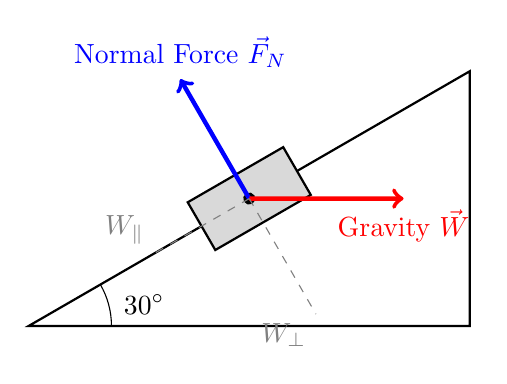
\begin{tikzpicture}[scale=0.7]
        % Inclined Plane
        \draw[thick] (0,0) -- (8,0) -- (8,4.62) -- cycle;
        \draw (1.5,0) arc (0:30:1.5) node[midway, right, xshift=2pt] {$30^\circ$};
        
        % Block Setup rotated to align with ramp
        \begin{scope}[shift={(4,2.31)}, rotate=30]
            \draw[thick, fill=gray!30] (-1,-0.5) rectangle (1,0.5);
            \draw[fill=black] (0,0) circle (0.1);
            % Forces
            \draw[->, ultra thick, blue] (0,0) -- (0,2.5) node[above] {Normal Force $\vec{F}_N$};
            \draw[->, ultra thick, red] (0,0) -- (-30:2.8) node[below] {Gravity $\vec{W}$};
            % Component lines
            \draw[dashed, gray] (0,0) -- (0,-2.42) node[below left] {$W_\perp$};
            \draw[dashed, gray] (0,0) -- (-2.0,0) node[above left] {$W_\parallel$};
        \end{scope}
    \end{tikzpicture}
    \end{center}
\end{enumerate}

